\documentclass[aspectratio=169]{beamer}

\setbeamersize{text margin left=5mm, text margin right=5mm}

\defbeamertemplate{headline}{my header}{%
\vskip1pt%
\makebox[0pt][l]{\,\insertshortauthor}%
\hspace*{\fill}\insertshorttitle/\insertshortsubtitle\hspace*{\fill}%
\llap{\insertpagenumber/\insertpresentationendpage\,}
}
\setbeamertemplate{headline}[my header]

\let\olditem\item
\renewcommand{\item}{\setlength{\itemsep}{\fill}\olditem}

\usepackage{caption}
\usepackage{soul}
\usepackage{tkz-euclide}
\usetikzlibrary{calc}
\usepackage[]{algorithm2e}
\usepackage{changepage}
\usepackage{amssymb}
\usepackage{xcolor}
\usepackage{mathtools}
\usepackage{tcolorbox}
\usepackage{tikz}
\usepackage{tikz-3dplot}
\usepackage{tkz-euclide}
\usepackage{circuitikz}
\usepackage{mleftright}
\usetikzlibrary{arrows.meta, decorations.pathreplacing, positioning, shapes.geometric}

%% Fonts
\usefonttheme{professionalfonts}
\usefonttheme{serif}

\DeclareCaptionLabelFormat{blank}{}
\captionsetup[figure]{labelformat=blank}

%% Math definitions
\def\mf{\ensuremath\mathbf}
\def\mb{\ensuremath\mathbb}
\def\mc{\ensuremath\mathcal}
\def\lp{\ensuremath\left(}
\def\rp{\ensuremath\right)}
\def\lv{\ensuremath\left\lvert}
\def\rv{\ensuremath\right\rvert}
\def\lV{\ensuremath\left\lVert}
\def\rV{\ensuremath\right\rVert}
\def\lc{\ensuremath\left\{}
\def\rc{\ensuremath\right\}}
\def\ls{\ensuremath\left[}
\def\rs{\ensuremath\right]}
\def\bmx{\ensuremath\begin{bmatrix*}[r]}
\def\emx{\ensuremath\end{bmatrix*}}
\def\bmxc{\ensuremath\begin{bmatrix*}[c]}
\def\t{\lp t\rp}
\def\k{\ls k\rs}

\newcommand{\demoex}[2]{\onslide<#1->\begin{color}{black!60} #2 \end{color}}
\newcommand{\demoexc}[3]{\onslide<#1->\begin{color}{#2} #3 \end{color}}
\newcommand{\anim}[3]{\onslide<#1->{\begin{color}{#2!60} #3 \end{color}}}
\newcommand{\ct}[1]{\lp #1\rp}
\newcommand{\dt}[1]{\ls #1\rs}
\newcommand{\cols}[2]{\begin{columns}[#1] #2 \end{columns}}
\newcommand{\col}[2]{\begin{column}{#1} #2 \end{column}}

%% Mycolors
\definecolor{myred}{RGB}{192,0,0}
\definecolor{mygray}{RGB}{100,100,100}

%% Custom beamer color
\setbeamercolor{title}{fg=myred}
\setbeamercolor{subtitle}{fg=myred}
\setbeamerfont{title}{series=\bfseries}
% \setbeamercolor{frametitle}{bg=myred, fg=white}
\setbeamercolor{frametitle}{bg=mygray!10!, fg=myred}
\setbeamerfont{frametitle}{series=\bfseries}
\setbeamercolor{item}{fg=mygray}
\setbeamercolor{title in head/foot}{fg=myred}

% Move header to footer
\setbeamertemplate{headline}{}
\setbeamertemplate{footline}{
  \begin{beamercolorbox}[wd=\paperwidth,ht=2.25ex,dp=1ex,center]{footline}
    \inserttitle\hfill\insertauthor\hfill\insertdate\hfill\insertframenumber{}
  \end{beamercolorbox}
}


\title{Applied Linear Algebra in Data Analysis}

% A subtitle is optional and this may be deleted
\subtitle{Application: Signal Processing}

\author{Sivakumar Balasubramanian}
% - Give the names in the same order as the appear in the paper.
% - Use the \inst{?} command only if the authors have different
%   affiliation.

\institute[Christian Medical College] % (optional, but mostly needed)
{
  \inst{}%
  Department of Bioengineering\\
  Christian Medical College, Bagayam\\
  Vellore 632002
}
% - Use the \inst command only if there are several affiliations.
% - Keep it simple, no one is interested in your street address.

\date{}
% - Either use conference name or its abbreviation.
% - Not really informative to the audience, more for people (including
%   yourself) who are reading the slides online

\subject{Lecture notes on ALADA}
% This is only inserted into the PDF information catalog. Can be left
% out. 

% If you have a file called "university-logo-filename.xxx", where xxx
% is a graphic format that can be processed by latex or pdflatex,
% resp., then you can add a logo as follows:

% \pgfdeclareimage[height=0.5cm]{university-logo}{university-logo-filename}
% \logo{\pgfuseimage{university-logo}}

% Delete this, if you do not want the table of contents to pop up at
% the beginning of each subsection:
\AtBeginSubsection[]
{
  \begin{frame}<beamer>{Outline}
    \tableofcontents[currentsection,currentsubsection]
  \end{frame}
}

% Let's get started
\begin{document}

\begin{frame}
  \titlepage
\end{frame}

% \begin{frame}[t]{References}
% \begin{itemize}
%   \item S Boyd, Applied Linear Algebra: Chapters 11.
%   \item G Strang, Linear Algebra: Chapters 1.
% \end{itemize}
% \end{frame}


\begin{frame}[t]{Signals as vectors}
  \textbf{What is a signal?} A \textit{signal} is a function of an independent variable that conveys some information.
  \begin{figure}[h]
    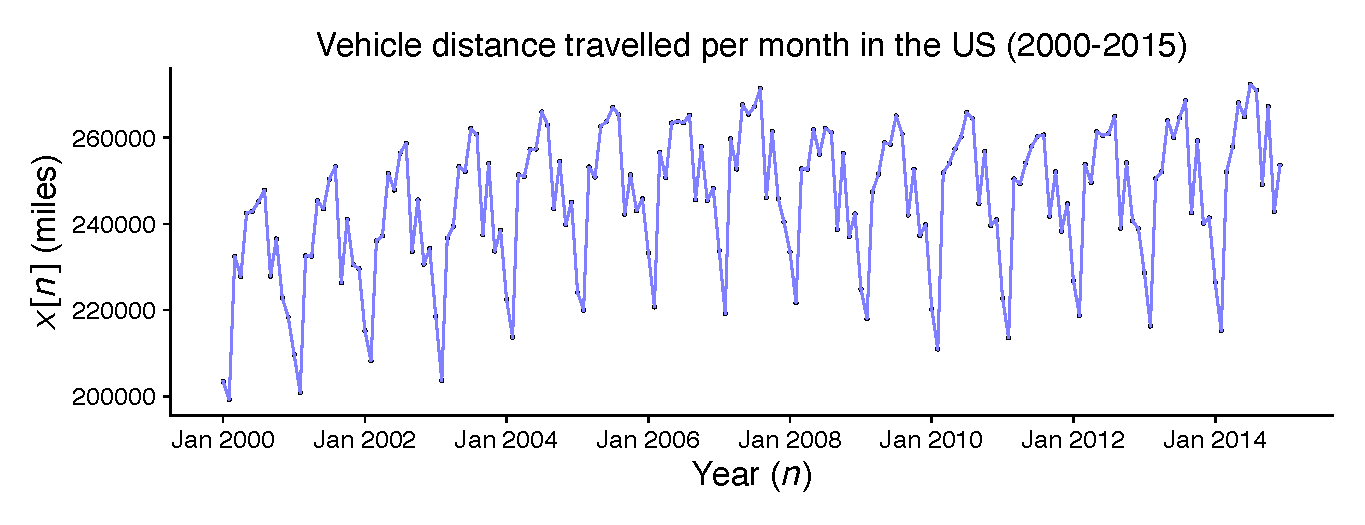
\includegraphics[width=1\textwidth]{figs/miles.eps}
  \end{figure}
\end{frame}


\begin{frame}[t]{Signals as vectors}
  \begin{figure}[h]
    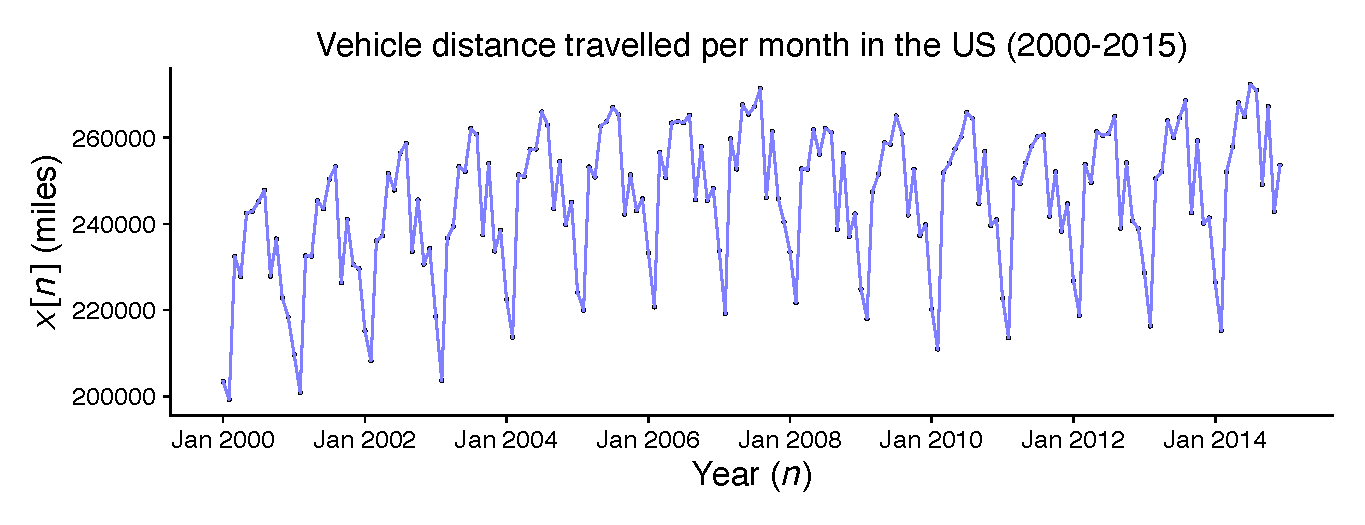
\includegraphics[width=0.6\textwidth]{figs/miles.eps}
  \end{figure}

  \begin{itemize}
    \item $x[n]$ in the above figure is a finite length signal of length $N$, where $n \in \mb{Z}, 0 \leq n < N$.
    \item We can think of signal as a vector $\mf{x}$ in $\mb{R}^N$, i.e. this entire signal will be a point in $N$-dimensional space. Here, $N= 180$.
    \[ \mf{x} = \bmx x[0] & x[1] & x[2] & \cdots & x[N-1]\emx^\top\]
  \end{itemize}
\end{frame}


\begin{frame}[t]{Signals as vectors}
  \begin{figure}[h]
    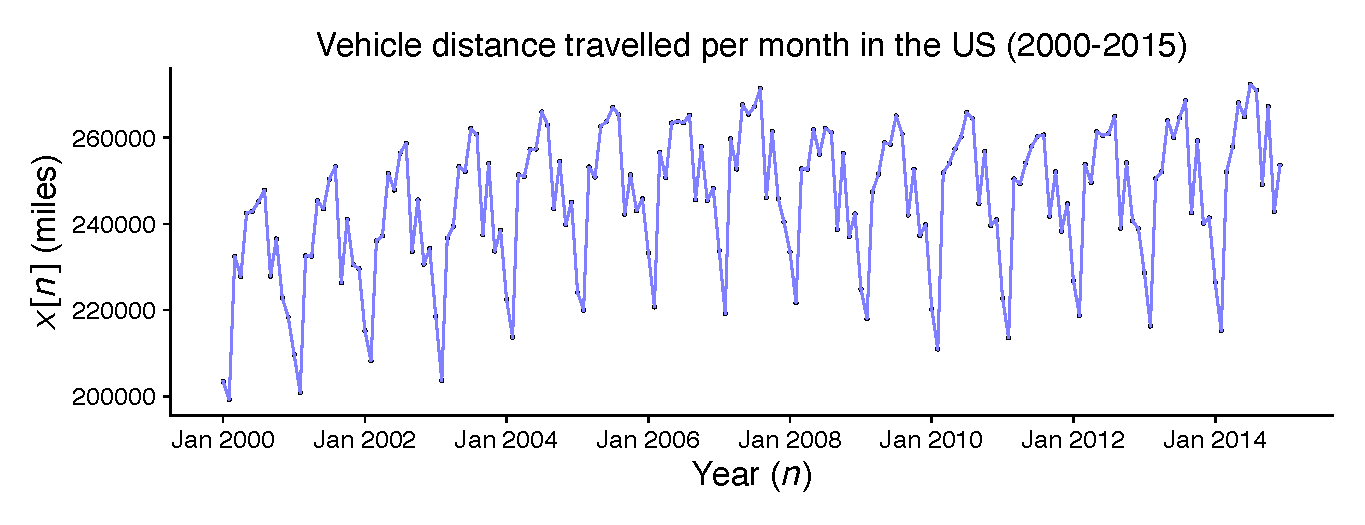
\includegraphics[width=0.6\textwidth]{figs/miles.eps}
  \end{figure}

  \begin{itemize}
    \item The above representation of $x[n]$ is in the standard basis $\lc \mf{e}_1, \mf{e}_2, \ldots \mf{e}_N\rc$.
    \[ \mf{x} = x[0] \cdot \mf{e}_1 + x[1] \cdot \mf{e}_2 + \cdots + x[N-1] \cdot \mf{e}_N \]

    \item What would this signal look like in a different basis?
  \end{itemize}
\end{frame}


\begin{frame}[t]{DFT: Fourier basis}
  \begin{itemize}
    \item For rhythmic signals, the Fourier basis is often useful. We will need to switch to the complex vector space $\mb{C}^N$ to work with the Fourier basis.
    
    \item Consider the following complex exponential signals of length $N$,
    \[
      \begin{split}
        w_k[n] &= e^{j \frac{2\pi k}{N}n}, \,\, 0 \leq n, k < N \\
               &= \cos\lp \frac{2\pi k}{N}n\rp + j \sin \lp \frac{2\pi k}{N}n\rp
      \end{split}
    \]

    We can represent this as a vector $\mf{w}_k \in \mb{C}^N$, where
    \[ \mf{w}_k = \bmx w_k[0] & w_k[1] & w_k[2] & \cdots & w_k[N-1] \emx^\top, \,\,\ 0 \leq k < N-1 \]
    
    There are $N$ such $\mf{w}_k$ vectors in $\mb{C}^N$.
  \end{itemize}
\end{frame}


\begin{frame}[t]{DFT: Fourier basis}
  \begin{itemize}
    \item The $\mf{w}_k$ vectors satisfy the following property,
    \[ \mf{w}_i^*\mf{w}_k = \begin{cases} N &, i = k \\ 0 &, i \neq k \end{cases} \]

    \item We define na orthonomgal basis for $\mb{C}^N$ as $\mc{F} = \lc \frac{1}{\sqrt{N}} \mf{w}_k \rc_{k=0}^{N-1}$.
    
    \item Using this orthonormal basis, we define the \textbf{Fourier matrix} as the following,
    \[ \mf{F}_N = \frac{1}{\sqrt{N}} \bmx \mf{w}_0 & \mf{w}_1 & \cdots & \mf{w}_{N-1} \emx \]

    \item It can be verified that $\mf{F}_N$ is a unitary matrix, i.e. $\mf{F}_N^H \mf{F}_N = \mf{I}_N$.
  \end{itemize}
\end{frame}


\begin{frame}[t]{DFT: Fourier basis}
  \begin{itemize}
    \item The representation of a signal $\mf{x}$ in the Fourier basis is given by,
    \[ \mf{x}_{\mc{F}} = \mf{F}_{N}^{-1} \mf{x} = \mf{F}_N^H \mf{x} \]

    $\mf{x}_{\mc{F}}$ representation is called the \textbf{Discrete Fourier Transform} (DFT) of $\mf{x}$.

    \item The inverse DFT, i.e. obtaining the $\mf{x}$ from $\mf{X}_{\mc{F}}$, is given by,
    \[ \mf{x} = \mf{F}_N \mf{x}_{\mc{F}} \]

    \item $\mf{x}$ is the called the \textit{time domain} representation of the signal, while $\mf{x}_{\mc{F}}$ is the \textit{frequency domain} representation of the signal.
  \end{itemize}
\end{frame}


\begin{frame}[t]{DFT: Fourier basis}
  \begin{itemize}
    \item The representation of a signal $\mf{x}$ in the Fourier basis is given by,
    \[ \mf{x}_{\mc{F}} = \mf{F}_{N}^{-1} \mf{x} = \mf{F}_N^H \mf{x} \]

    $\mf{x}_{\mc{F}}$ representation is called the \textbf{Discrete Fourier Transform} (DFT) of $\mf{x}$.

    \item The inverse DFT, i.e. obtaining the $\mf{x}$ from $\mf{X}_{\mc{F}}$, is given by,
    \[ \mf{x} = \mf{F}_N \mf{x}_{\mc{F}} \]

    \item $\mf{x}$ is the called the \textit{time domain} representation of the signal, while $\mf{x}_{\mc{F}}$ is the \textit{frequency domain} representation of the signal.
  \end{itemize}
\end{frame}


\begin{frame}[t]{Frequency domain representation of $x[n]$}
  \begin{figure}[h]
    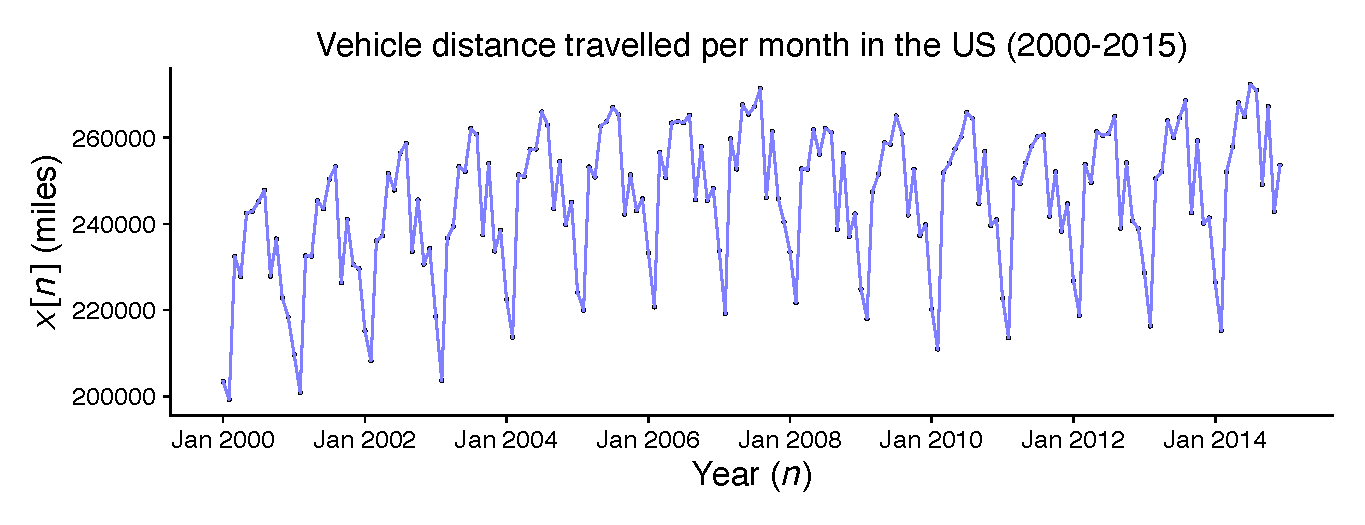
\includegraphics[width=0.4\textwidth]{figs/miles.eps}
  \end{figure}

  \begin{figure}[h]
    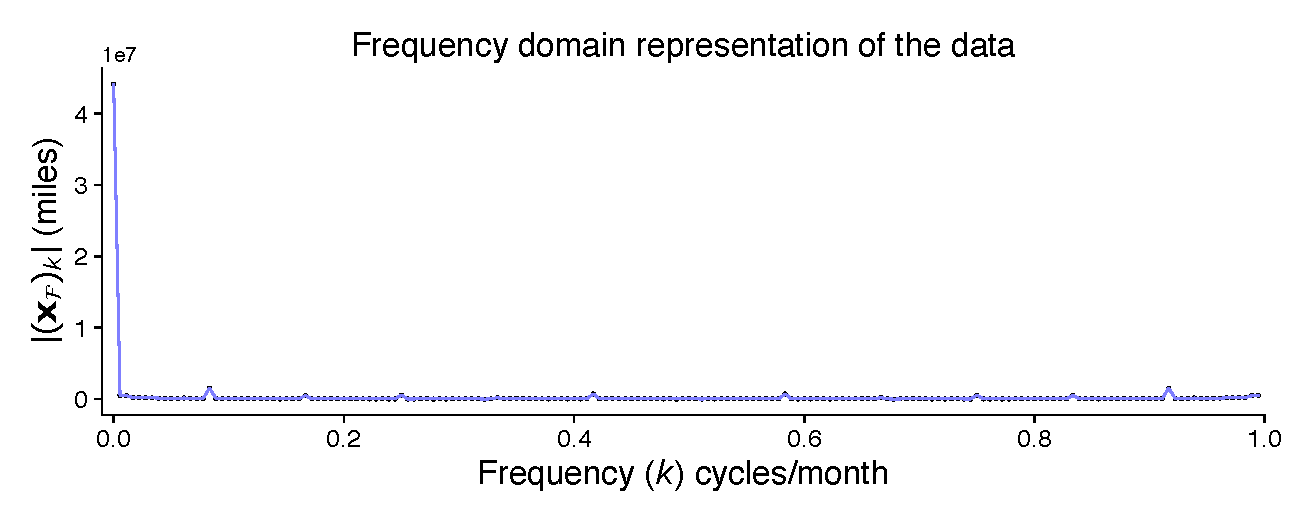
\includegraphics[width=0.9\textwidth]{figs/miles_fft.eps}
  \end{figure}
\end{frame}


\begin{frame}[t]{Frequency domain representation of $x[n]$}
  Real and Imaginary components
  \begin{figure}[h]
    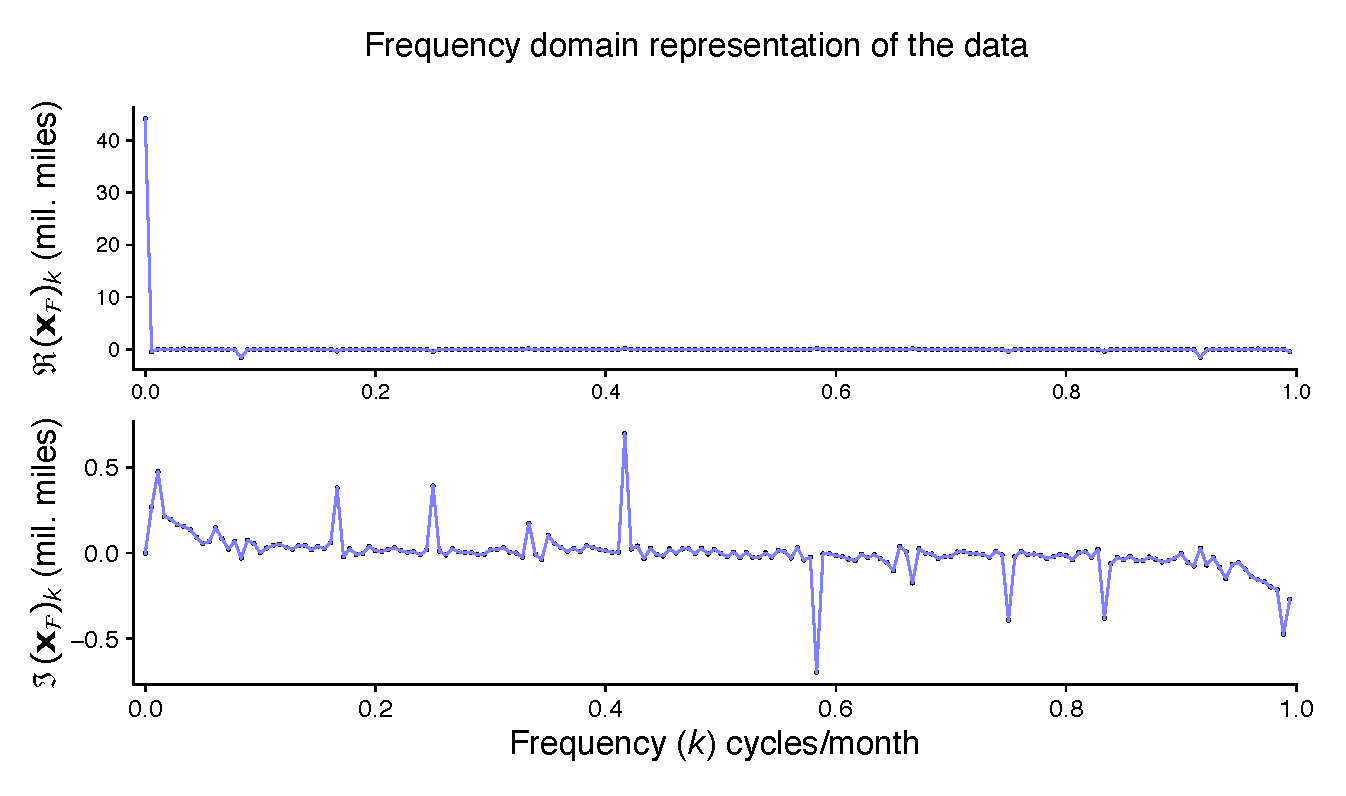
\includegraphics[width=0.8\textwidth]{figs/miles_fft_reim.eps}
  \end{figure}
\end{frame}


\begin{frame}[t]{Frequency domain representation of mean subtracted $x[n]$}
  \begin{figure}[h]
    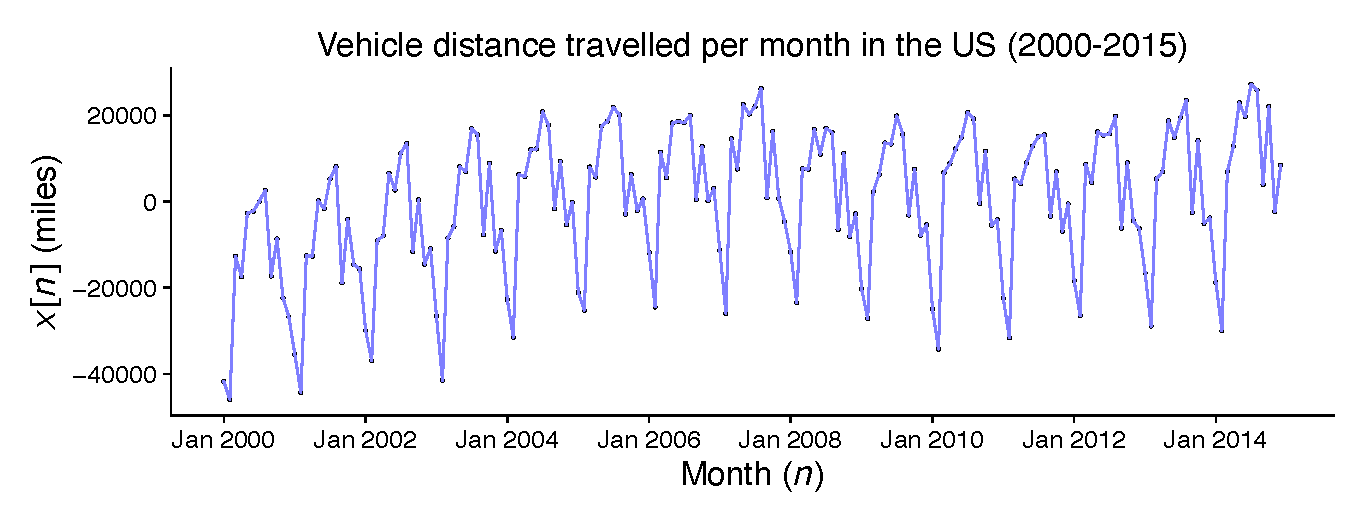
\includegraphics[width=0.4\textwidth]{figs/miles_nomean.eps}
  \end{figure}

  \begin{figure}[h]
    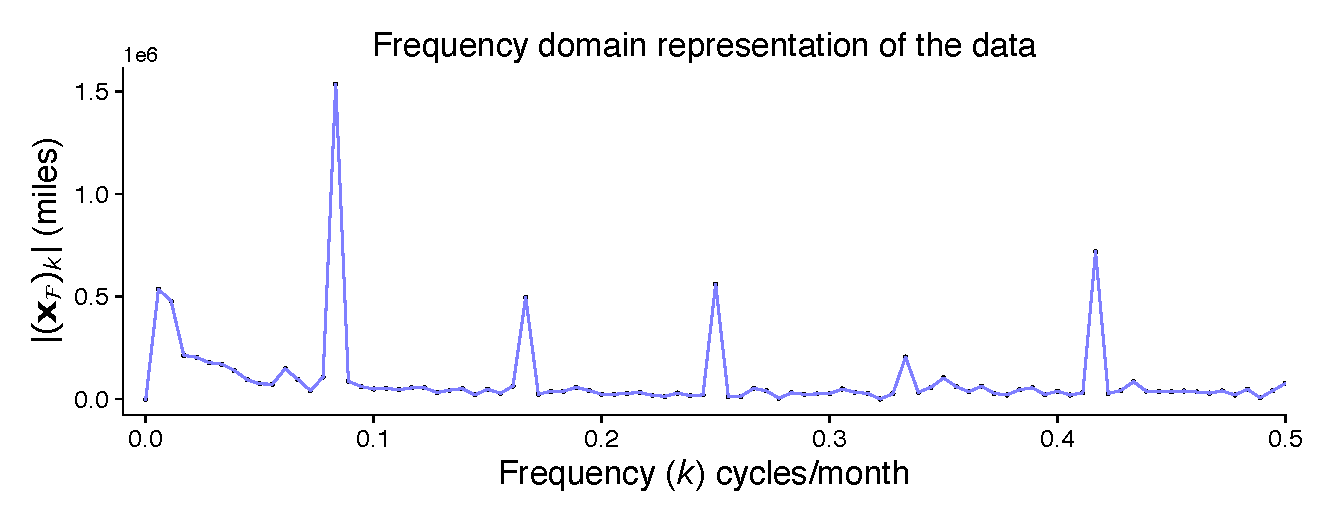
\includegraphics[width=0.9\textwidth]{figs/miles_nomean_fft.eps}
  \end{figure}
\end{frame}


\begin{frame}[t]{Frequency domain representation of mean subtracted $x[n]$}
  Real and Imaginary components
  \begin{figure}[h]
    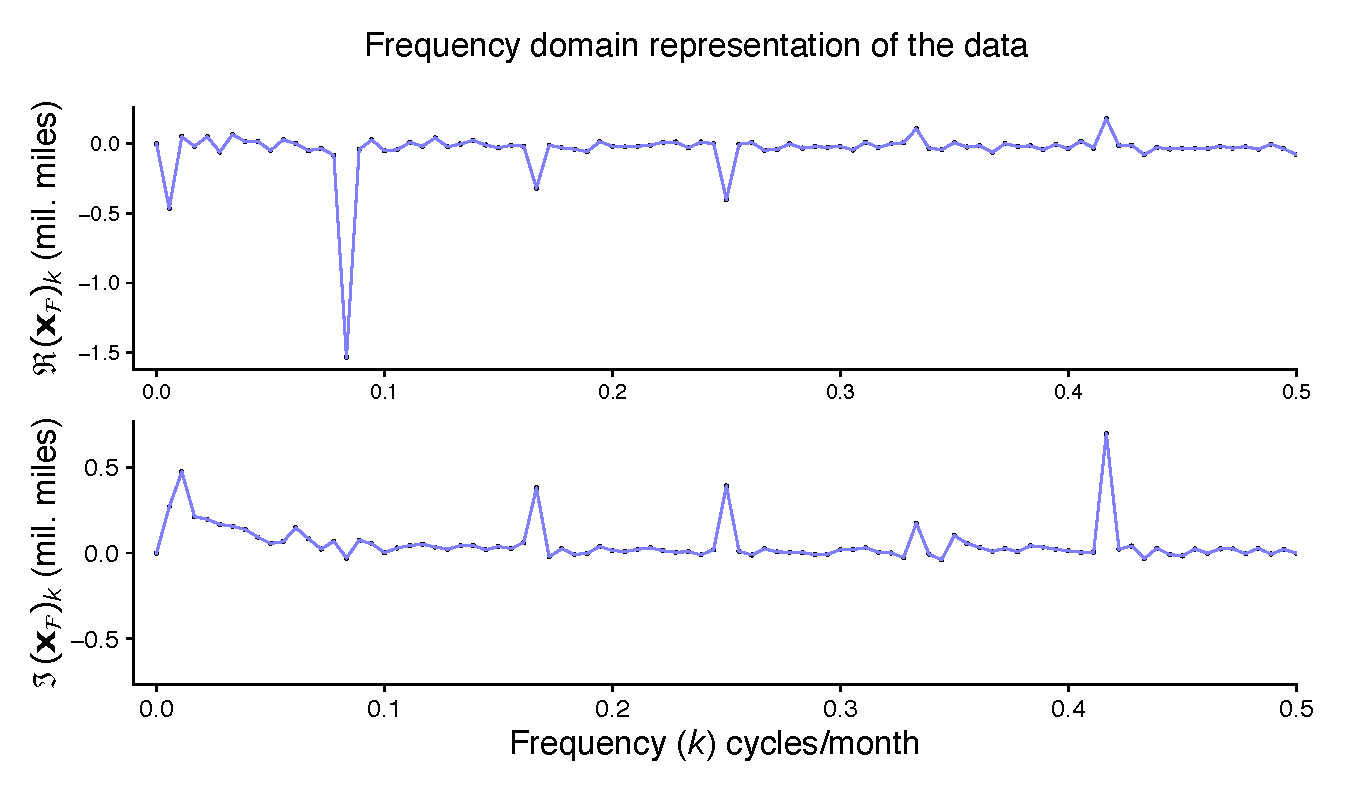
\includegraphics[width=0.8\textwidth]{figs/miles_nomean_fft_reim.eps}
  \end{figure}
\end{frame}


\begin{frame}[t]{Problems with the Fourier basis}
  Fourier basis is not suitable for representing transient signals. They are not localized in time.
  \begin{figure}[h]
    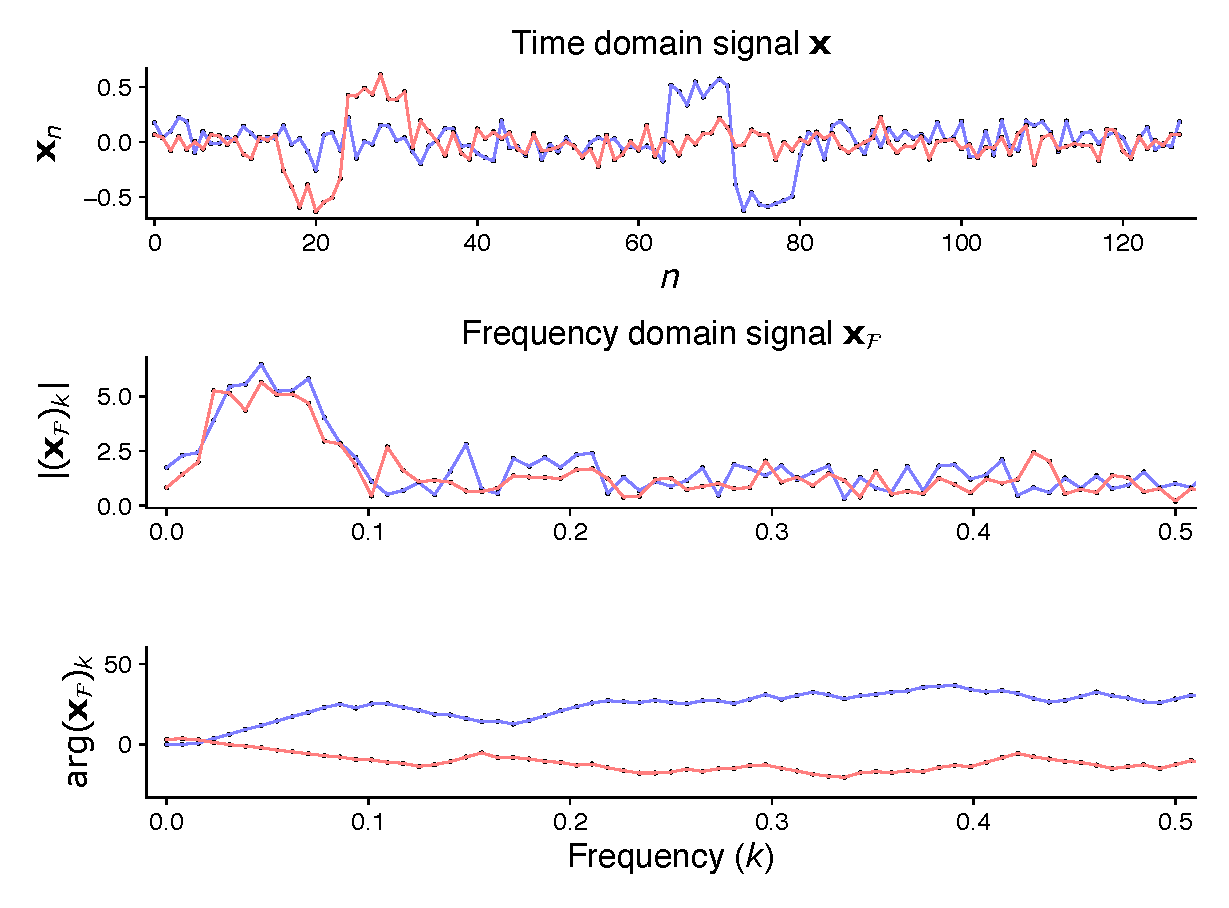
\includegraphics[width=0.6\textwidth]{figs/signal_transient.eps}
  \end{figure}
\end{frame}


\begin{frame}[t]{Wavelet basis}
  Wavelet basis are localized in time and frequency, making them suitable for transient signals.
  
  The \textbf{Haar wavelet} is the simplest wavelet basis. Consider a the vector space $\mb{R}^8$, the Haar wavelet basis $\mc{W} = \lc \mf{h}_k \rc_{k=1}^8$ for this space is given by,
  \[ \scriptscriptstyle \mf{h}_1 = \frac{1}{\sqrt{8}}\bmx 1 \\ 1 \\ 1 \\ 1 \\ 1 \\ 1 \\ 1 \\ 1 \emx \,\, 
  \mf{h}_2 = \frac{1}{\sqrt{8}}\bmx 1 \\ 1 \\ 1 \\ 1 \\ -1 \\ -1 \\ -1 \\ -1 \emx \,\, 
  \mf{h}_3 = \frac{1}{2}\bmx 1 \\ 1 \\ -1 \\ -1 \\ 0 \\ 0 \\ 0 \\ 0 \emx \,\, 
  \mf{h}_4 = \frac{1}{2}\bmx 0 \\ 0 \\ 0 \\ 0 \\ 1 \\ 1 \\ -1 \\ -1 \emx \,\, 
  \mf{h}_5 = \frac{1}{\sqrt{2}}\bmx 1 \\ -1 \\ 0 \\ 0 \\ 0 \\ 0 \\ 0 \\ 0 \emx \,\, 
  \mf{h}_6 = \frac{1}{\sqrt{2}}\bmx 0 \\ 0 \\ 1 \\ -1 \\ 0 \\ 0 \\ 0 \\ 0 \emx \,\, 
  \mf{h}_7 = \frac{1}{\sqrt{2}}\bmx 0 \\ 0 \\ 0 \\ 0 \\ 1 \\ -1 \\ 0 \\ 0 \emx \,\, 
  \mf{h}_8 = \frac{1}{\sqrt{2}}\bmx 0 \\ 0 \\ 0 \\ 0 \\ 0 \\ 0 \\ 1 \\ -1 \emx 
  \]
  \[ \mf{W}_8 = \bmx \mf{h}_1 & \mf{h}_2 & \mf{h}_3 & \mf{h}_4 & \mf{h}_5 & \mf{h}_6 & \mf{h}_7 & \mf{h}_8 \emx\]
\end{frame}


\begin{frame}[t]{Wavelet basis}
  \begin{columns}[T]
    \begin{column}{0.45\textwidth}
      The wavelet basis is a an orthonormal basis for $\mb{R}^8$.
      \[  \mf{W}_8^H \mf{W}_8 = \mf{I} \]

      Let $x[n], \,\, 0 \leq n < 8$ be a signal of length $8$, which can represented in the standard basis of $\mb{R}^8$ as,
      \[ \mf{x} = \bmx x[0] & x[1] & x[2] & \cdots & x[7] \emx^\top \]

      The resentation of this signal is the wavelet basis is given by,
      \[ \mf{x}_{\mc{W}} = \mf{W}_8^{-1} \mf{x} = \mf{W}_8^{\top} \mf{x}\]

    \end{column}
    \begin{column}{0.52\textwidth}
      \vspace{-1cm}
      \begin{figure}[t]
        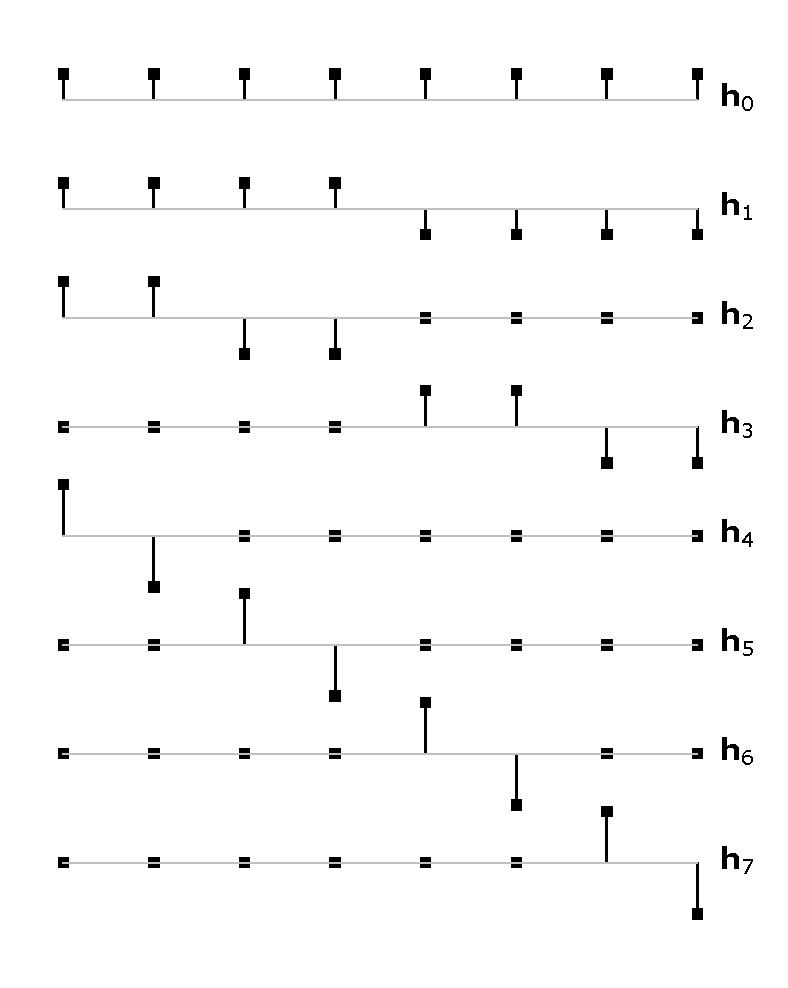
\includegraphics[width=0.85\textwidth]{figs/haar_vectors.eps}
      \end{figure}
    \end{column}
  \end{columns}
\end{frame}


\begin{frame}[t]{Represention in the wavelet basis}
  \begin{figure}[t]
    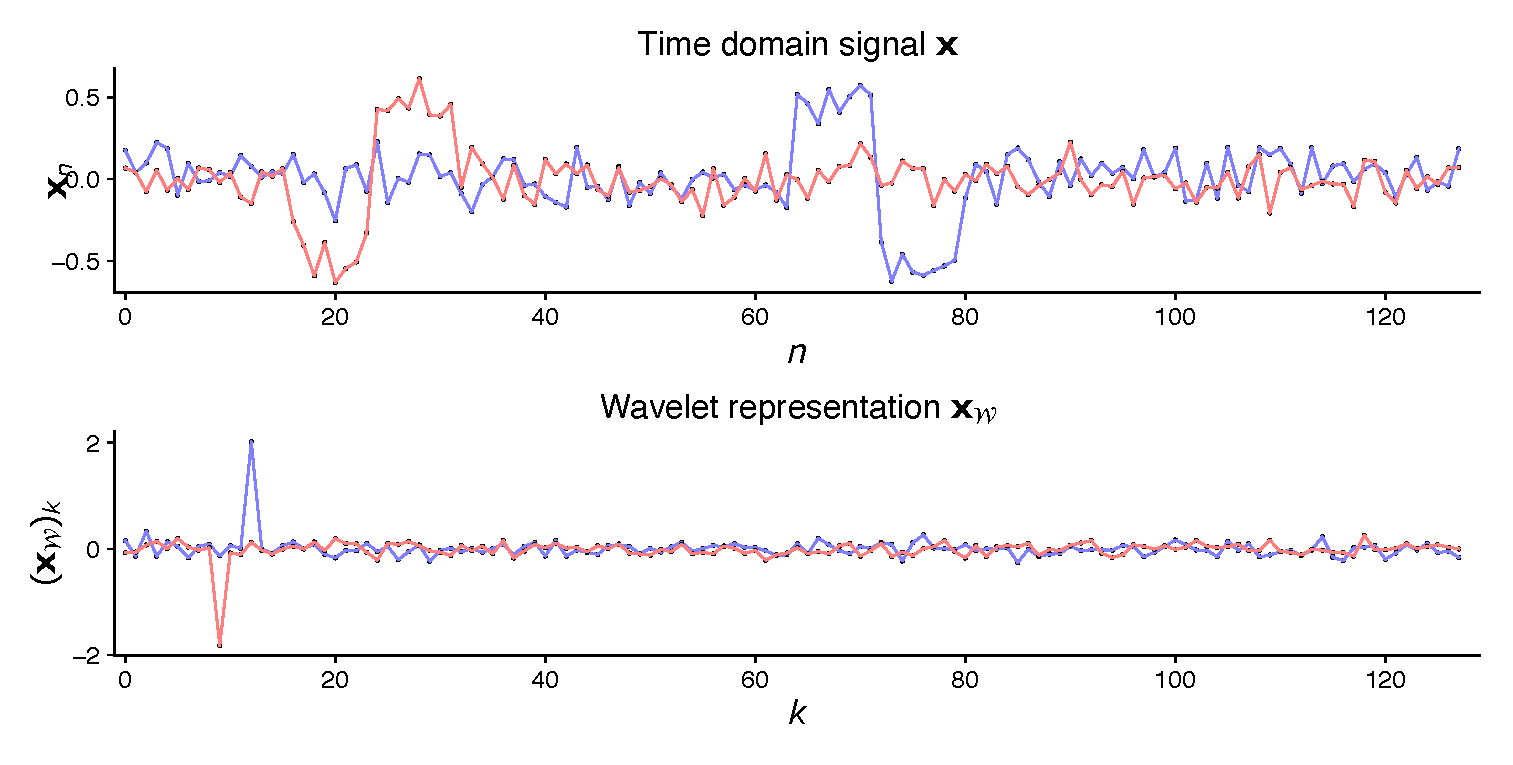
\includegraphics[width=0.85\textwidth]{figs/signal_transient_wavedec.eps}
  \end{figure}
  \vspace{-0.25cm}

  The Haar wavelet provides a sparse representation of the red and blue signals, because they are well matched with the Haar bases.
\end{frame}


\begin{frame}[t]{Represention in the wavelet basis}
  \begin{figure}[t]
    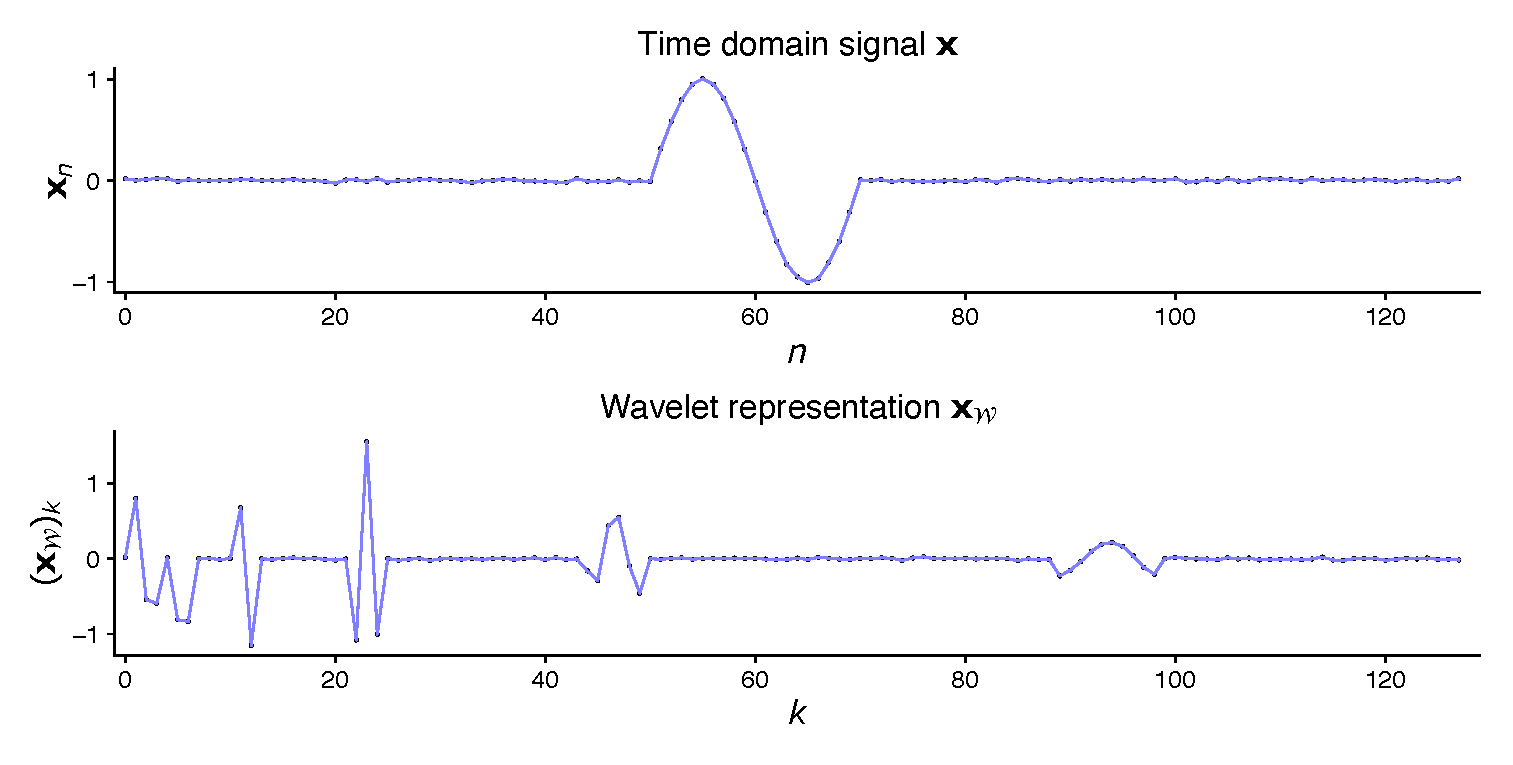
\includegraphics[width=0.85\textwidth]{figs/sine_transient_wavedec.eps}
  \end{figure}
  \vspace{-0.25cm}
  
  When the signal is not well matched with the wavelet basis, the representation is not sparse or less sparse.
\end{frame}


\end{document}